
%(BEGIN_QUESTION)
% Copyright 2006, Tony R. Kuphaldt, released under the Creative Commons Attribution License (v 1.0)
% This means you may do almost anything with this work of mine, so long as you give me proper credit

Fullfør kalibreringstabellen for denne strømningsmålesløyfen, som består av en orificeplate, $\Delta$P-transmitter, kvadratrotekstraktor og indikator.  Anta følgende instrumentområder:

$$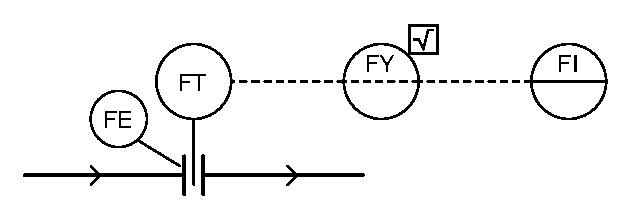
\includegraphics[width=15.5cm]{i00048x01.eps}$$

\begin{itemize}
\item{} FE: 0-750 GPM, 0-100 "W.C. $\Delta$P
\item{} FT: 0-100 "W.C. inn, 4-20 mA ut (lineær)
\item{} FY: 4-20 mA inn og ut (kvadratroten)
\item{} FI: 4-20 mA inn, 0-750 GPM indikasjon
\end{itemize}

% No blank lines allowed between lines of an \halign structure!
% I use comments (%) instead, so that TeX doesn't choke.

$$\vbox{\offinterlineskip
\halign{\strut
\vrule \quad\hfil # \ \hfil & 
\vrule \quad\hfil # \ \hfil & 
\vrule \quad\hfil # \ \hfil & 
\vrule \quad\hfil # \ \hfil & 
\vrule \quad\hfil # \ \hfil & 
\vrule \quad\hfil # \ \hfil \vrule \cr
\noalign{\hrule}
%
% First row
Strømningsrate & Prosent av & Orifice $\Delta$P & FT-utgang & FY-utgang & FI-indikasjon \cr
%
% Another row
(GPM) & maks. flow (\%) & ("W.C.) & signal (mA) & signal (mA) & (GPM) \cr
%
\noalign{\hrule}
%
% Another row
0 & 0 &   &   &   & 0 \cr
%
\noalign{\hrule}
%
% Another row
  & 10 &   &   &   &  \cr
%
\noalign{\hrule}
%
% Another row
  & 25 &   &   &   &  \cr
%
\noalign{\hrule}
%
% Another row
375 & 50 &   &   &   & 375 \cr
%
\noalign{\hrule}
%
% Another row
  & 75 &   &   &   &  \cr
%
\noalign{\hrule}
%
% Another row
  & 90 &   &   &   &  \cr
%
\noalign{\hrule}
%
% Another row
750 & 100 &   &   &   & 750 \cr
%
\noalign{\hrule}
} % End of \halign 
}$$ % End of \vbox

\vfil

\underbar{file i00048}
\eject
%(END_QUESTION)





%(BEGIN_ANSWER)

Dette er et vurdert spørsmål -- ingen svar eller hint gis!

%(END_ANSWER)





%(BEGIN_NOTES)

% No blank lines allowed between lines of an \halign structure!
% I use comments (%) instead, so that TeX doesn't choke.

$$\vbox{\offinterlineskip
\halign{\strut
\vrule \quad\hfil # \ \hfil & 
\vrule \quad\hfil # \ \hfil & 
\vrule \quad\hfil # \ \hfil & 
\vrule \quad\hfil # \ \hfil & 
\vrule \quad\hfil # \ \hfil & 
\vrule \quad\hfil # \ \hfil \vrule \cr
\noalign{\hrule}
%
% First row
Strømningsrate & Prosent av & Orifice $\Delta$P & FT-utgang & FY-utgang & FI-indikasjon \cr
%
% Another row
(GPM) & maks. flow (\%) & ("W.C.) & signal (mA) & signal (mA) & (GPM) \cr
%
\noalign{\hrule}
%
% Another row
0 & 0 & 0 & 4 & 4 & 0 \cr
%
\noalign{\hrule}
%
% Another row
75  & 10 & 1 & 4.16 & 5.6 & 75 \cr
%
\noalign{\hrule}
%
% Another row
187.5  & 25 & 6.25 & 5 & 8 & 187.5 \cr
%
\noalign{\hrule}
%
% Another row
375 & 50 & 25 & 8 & 12 & 375 \cr
%
\noalign{\hrule}
%
% Another row
562.5 & 75 & 56.25 & 13 & 16 & 562.5 \cr
%
\noalign{\hrule}
%
% Another row
675 & 90 & 81 & 16.96 & 18.4 & 675 \cr
%
\noalign{\hrule}
%
% Another row
750 & 100 & 100 & 20 & 20 & 750 \cr
%
\noalign{\hrule}
} % End of \halign 
}$$ % End of \vbox

Konvertering av prosentverdier til strømningsrater er enkelt: multipliser hver prosent med maksimal (URV) strømningsrate.

\vskip 10pt

Å konvertere prosentverdier til differansetrykk er litt mer krevende.  Siden orificeplaten er iboende ikke-lineær -- den genererer differansetrykk proporsjonalt med {\it kvadratet} av strømningsraten -- må vi ta prosent av flow og deretter kvadrere den prosenten for å få prosent av DP.  Denne nye (kvadrerte) prosentverdien multipliseres så med URV i trykkområdet for å beregne DP.

\vskip 10pt

Flowtransmitteren er lineær, og den tar bare målt DP og konverterer det lineært til et milliamp-signal.

\vskip 10pt

Kvadratrotekstraktoren (reléet) tar inn transmitterens milliamp-signal, kvadratroter signalprosenten, og genererer deretter sitt eget milliamp-signal som representerer prosent av flow.  Sluttresultatet er at reléets milliamp-signal er lineært i forhold til faktisk strømningsrate.

%INDEX% Calibration: table, flow transmitter
%INDEX% Measurement, flow: calibration table

%(END_NOTES)
